\documentclass[10pt]{standalone}
\usepackage[utf8]{inputenc}
\usepackage{pgfplots}
\pgfplotsset{compat=1.15}
\usepackage{mathrsfs}
\usetikzlibrary{arrows}
\pagestyle{empty}
\begin{document}

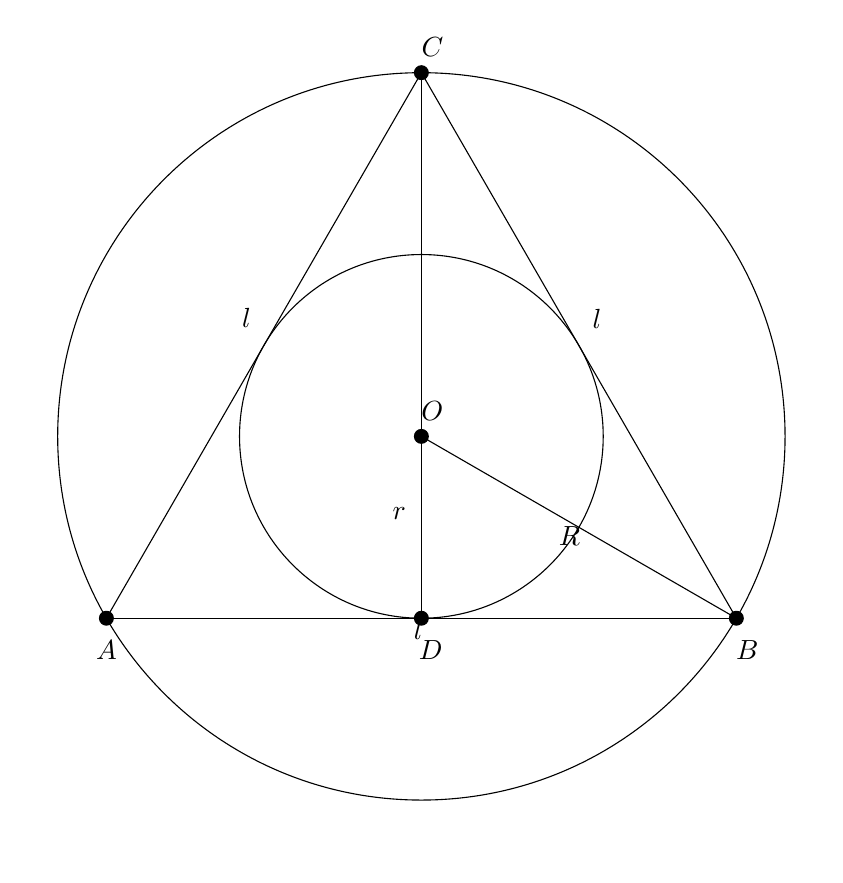
\begin{tikzpicture}[line cap=round,line join=round,>=triangle 45,x=1.0cm,y=1.0cm]
\clip(-5.,-2.) rectangle (5.,8.5);
\draw  (-4.,1.)-- (4.,1.);
\draw  (0.,7.928203230275509)-- (4.,1.);
\draw  (0.,7.928203230275509)-- (-4.,1.);
\draw  (0.,3.309401076758503) circle (2.309401076758503cm);
\draw  (0.,3.309401076758503)-- (0.,1.);
\draw  (0.,7.928203230275509)-- (0.,3.309401076758503);
\draw  (0.,3.309401076758503)-- (4.,1.);
\draw  (0.,3.309401076758503) circle (4.618802153517006cm);

\draw [fill=black] (-4.,1.) circle (2.5pt);
\draw[color=black] (-4.0,0.6) node {$A$};
\draw [fill=black] (4.,1.) circle (2.5pt);
\draw[color=black] (4.14,0.6) node {$B$};
\draw[color=black] (-0.04,0.85) node {$l$};
\draw [fill=black] (0.,-5.92820323027551) circle (2.5pt);
%\draw[color=black] (-11.47,11.34) node {$C_{1}$};
\draw [fill=black] (0.,7.928203230275509) circle (2.5pt);
\draw[color=black] (0.14,8.25) node {$C$};
\draw[color=black] (2.23,4.8) node {$l$};
\draw[color=black] (-2.22,4.81) node {$l$};
\draw [fill=black] (0.,3.309401076758503) circle (2.5pt);
\draw[color=black] (0.14,3.63) node {$O$};
\draw [fill=black] (0.,1.) circle (2.5pt);
\draw[color=black] (0.12,0.6) node {$D$};
\draw[color=black] (-0.28,2.33) node {$r$};
\draw[color=black] (1.88,2.05) node {$R$};

\end{tikzpicture}
\end{document}